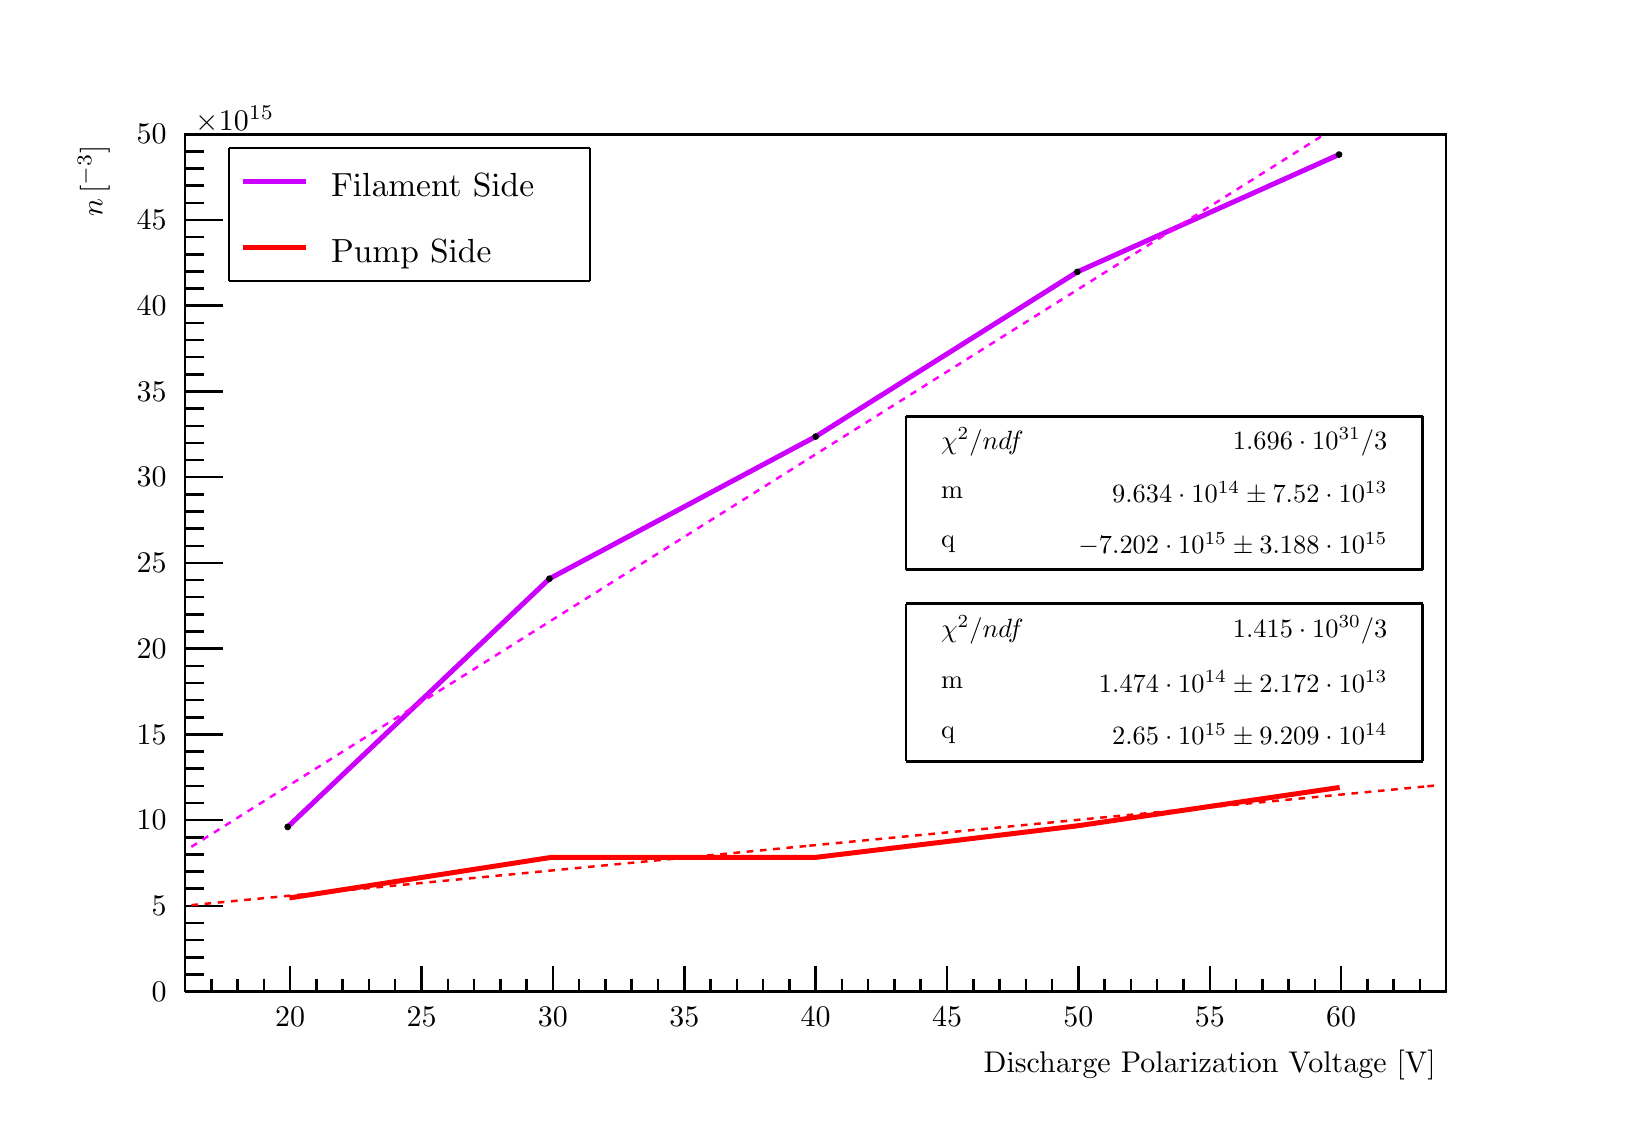
\begin{tikzpicture}
\pgfdeclareplotmark{cross} {
\pgfpathmoveto{\pgfpoint{-0.3\pgfplotmarksize}{\pgfplotmarksize}}
\pgfpathlineto{\pgfpoint{+0.3\pgfplotmarksize}{\pgfplotmarksize}}
\pgfpathlineto{\pgfpoint{+0.3\pgfplotmarksize}{0.3\pgfplotmarksize}}
\pgfpathlineto{\pgfpoint{+1\pgfplotmarksize}{0.3\pgfplotmarksize}}
\pgfpathlineto{\pgfpoint{+1\pgfplotmarksize}{-0.3\pgfplotmarksize}}
\pgfpathlineto{\pgfpoint{+0.3\pgfplotmarksize}{-0.3\pgfplotmarksize}}
\pgfpathlineto{\pgfpoint{+0.3\pgfplotmarksize}{-1.\pgfplotmarksize}}
\pgfpathlineto{\pgfpoint{-0.3\pgfplotmarksize}{-1.\pgfplotmarksize}}
\pgfpathlineto{\pgfpoint{-0.3\pgfplotmarksize}{-0.3\pgfplotmarksize}}
\pgfpathlineto{\pgfpoint{-1.\pgfplotmarksize}{-0.3\pgfplotmarksize}}
\pgfpathlineto{\pgfpoint{-1.\pgfplotmarksize}{0.3\pgfplotmarksize}}
\pgfpathlineto{\pgfpoint{-0.3\pgfplotmarksize}{0.3\pgfplotmarksize}}
\pgfpathclose
\pgfusepathqstroke
}
\pgfdeclareplotmark{cross*} {
\pgfpathmoveto{\pgfpoint{-0.3\pgfplotmarksize}{\pgfplotmarksize}}
\pgfpathlineto{\pgfpoint{+0.3\pgfplotmarksize}{\pgfplotmarksize}}
\pgfpathlineto{\pgfpoint{+0.3\pgfplotmarksize}{0.3\pgfplotmarksize}}
\pgfpathlineto{\pgfpoint{+1\pgfplotmarksize}{0.3\pgfplotmarksize}}
\pgfpathlineto{\pgfpoint{+1\pgfplotmarksize}{-0.3\pgfplotmarksize}}
\pgfpathlineto{\pgfpoint{+0.3\pgfplotmarksize}{-0.3\pgfplotmarksize}}
\pgfpathlineto{\pgfpoint{+0.3\pgfplotmarksize}{-1.\pgfplotmarksize}}
\pgfpathlineto{\pgfpoint{-0.3\pgfplotmarksize}{-1.\pgfplotmarksize}}
\pgfpathlineto{\pgfpoint{-0.3\pgfplotmarksize}{-0.3\pgfplotmarksize}}
\pgfpathlineto{\pgfpoint{-1.\pgfplotmarksize}{-0.3\pgfplotmarksize}}
\pgfpathlineto{\pgfpoint{-1.\pgfplotmarksize}{0.3\pgfplotmarksize}}
\pgfpathlineto{\pgfpoint{-0.3\pgfplotmarksize}{0.3\pgfplotmarksize}}
\pgfpathclose
\pgfusepathqfillstroke
}
\pgfdeclareplotmark{newstar} {
\pgfpathmoveto{\pgfqpoint{0pt}{\pgfplotmarksize}}
\pgfpathlineto{\pgfqpointpolar{44}{0.5\pgfplotmarksize}}
\pgfpathlineto{\pgfqpointpolar{18}{\pgfplotmarksize}}
\pgfpathlineto{\pgfqpointpolar{-20}{0.5\pgfplotmarksize}}
\pgfpathlineto{\pgfqpointpolar{-54}{\pgfplotmarksize}}
\pgfpathlineto{\pgfqpointpolar{-90}{0.5\pgfplotmarksize}}
\pgfpathlineto{\pgfqpointpolar{234}{\pgfplotmarksize}}
\pgfpathlineto{\pgfqpointpolar{198}{0.5\pgfplotmarksize}}
\pgfpathlineto{\pgfqpointpolar{162}{\pgfplotmarksize}}
\pgfpathlineto{\pgfqpointpolar{134}{0.5\pgfplotmarksize}}
\pgfpathclose
\pgfusepathqstroke
}
\pgfdeclareplotmark{newstar*} {
\pgfpathmoveto{\pgfqpoint{0pt}{\pgfplotmarksize}}
\pgfpathlineto{\pgfqpointpolar{44}{0.5\pgfplotmarksize}}
\pgfpathlineto{\pgfqpointpolar{18}{\pgfplotmarksize}}
\pgfpathlineto{\pgfqpointpolar{-20}{0.5\pgfplotmarksize}}
\pgfpathlineto{\pgfqpointpolar{-54}{\pgfplotmarksize}}
\pgfpathlineto{\pgfqpointpolar{-90}{0.5\pgfplotmarksize}}
\pgfpathlineto{\pgfqpointpolar{234}{\pgfplotmarksize}}
\pgfpathlineto{\pgfqpointpolar{198}{0.5\pgfplotmarksize}}
\pgfpathlineto{\pgfqpointpolar{162}{\pgfplotmarksize}}
\pgfpathlineto{\pgfqpointpolar{134}{0.5\pgfplotmarksize}}
\pgfpathclose
\pgfusepathqfillstroke
}
\definecolor{c}{rgb}{1,1,1};
\draw [color=c, fill=c] (0,0) rectangle (20,13.6103);
\draw [color=c, fill=c] (1.9914,1.37536) rectangle (18.0086,12.2636);
\definecolor{c}{rgb}{0,0,0};
\draw [c,line width=0.9] (1.9914,1.37536) -- (1.9914,12.2636) -- (18.0086,12.2636) -- (18.0086,1.37536) -- (1.9914,1.37536);
\definecolor{c}{rgb}{1,1,1};
\draw [color=c, fill=c] (1.9914,1.37536) rectangle (18.0086,12.2636);
\definecolor{c}{rgb}{0,0,0};
\draw [c,line width=0.9] (1.9914,1.37536) -- (1.9914,12.2636) -- (18.0086,12.2636) -- (18.0086,1.37536) -- (1.9914,1.37536);
\draw [c,line width=0.9] (1.9914,1.37536) -- (18.0086,1.37536);
\draw [c,line width=0.9] (3.32617,1.70236) -- (3.32617,1.37536);
\draw [c,line width=0.9] (3.65986,1.53886) -- (3.65986,1.37536);
\draw [c,line width=0.9] (3.99355,1.53886) -- (3.99355,1.37536);
\draw [c,line width=0.9] (4.32724,1.53886) -- (4.32724,1.37536);
\draw [c,line width=0.9] (4.66094,1.53886) -- (4.66094,1.37536);
\draw [c,line width=0.9] (4.99463,1.70236) -- (4.99463,1.37536);
\draw [c,line width=0.9] (5.32832,1.53886) -- (5.32832,1.37536);
\draw [c,line width=0.9] (5.66201,1.53886) -- (5.66201,1.37536);
\draw [c,line width=0.9] (5.9957,1.53886) -- (5.9957,1.37536);
\draw [c,line width=0.9] (6.32939,1.53886) -- (6.32939,1.37536);
\draw [c,line width=0.9] (6.66308,1.70236) -- (6.66308,1.37536);
\draw [c,line width=0.9] (6.99678,1.53886) -- (6.99678,1.37536);
\draw [c,line width=0.9] (7.33047,1.53886) -- (7.33047,1.37536);
\draw [c,line width=0.9] (7.66416,1.53886) -- (7.66416,1.37536);
\draw [c,line width=0.9] (7.99785,1.53886) -- (7.99785,1.37536);
\draw [c,line width=0.9] (8.33154,1.70236) -- (8.33154,1.37536);
\draw [c,line width=0.9] (8.66523,1.53886) -- (8.66523,1.37536);
\draw [c,line width=0.9] (8.99893,1.53886) -- (8.99893,1.37536);
\draw [c,line width=0.9] (9.33262,1.53886) -- (9.33262,1.37536);
\draw [c,line width=0.9] (9.66631,1.53886) -- (9.66631,1.37536);
\draw [c,line width=0.9] (10,1.70236) -- (10,1.37536);
\draw [c,line width=0.9] (10.3337,1.53886) -- (10.3337,1.37536);
\draw [c,line width=0.9] (10.6674,1.53886) -- (10.6674,1.37536);
\draw [c,line width=0.9] (11.0011,1.53886) -- (11.0011,1.37536);
\draw [c,line width=0.9] (11.3348,1.53886) -- (11.3348,1.37536);
\draw [c,line width=0.9] (11.6685,1.70236) -- (11.6685,1.37536);
\draw [c,line width=0.9] (12.0021,1.53886) -- (12.0021,1.37536);
\draw [c,line width=0.9] (12.3358,1.53886) -- (12.3358,1.37536);
\draw [c,line width=0.9] (12.6695,1.53886) -- (12.6695,1.37536);
\draw [c,line width=0.9] (13.0032,1.53886) -- (13.0032,1.37536);
\draw [c,line width=0.9] (13.3369,1.70236) -- (13.3369,1.37536);
\draw [c,line width=0.9] (13.6706,1.53886) -- (13.6706,1.37536);
\draw [c,line width=0.9] (14.0043,1.53886) -- (14.0043,1.37536);
\draw [c,line width=0.9] (14.338,1.53886) -- (14.338,1.37536);
\draw [c,line width=0.9] (14.6717,1.53886) -- (14.6717,1.37536);
\draw [c,line width=0.9] (15.0054,1.70236) -- (15.0054,1.37536);
\draw [c,line width=0.9] (15.3391,1.53886) -- (15.3391,1.37536);
\draw [c,line width=0.9] (15.6728,1.53886) -- (15.6728,1.37536);
\draw [c,line width=0.9] (16.0064,1.53886) -- (16.0064,1.37536);
\draw [c,line width=0.9] (16.3401,1.53886) -- (16.3401,1.37536);
\draw [c,line width=0.9] (16.6738,1.70236) -- (16.6738,1.37536);
\draw [c,line width=0.9] (3.32617,1.70236) -- (3.32617,1.37536);
\draw [c,line width=0.9] (2.99248,1.53886) -- (2.99248,1.37536);
\draw [c,line width=0.9] (2.65879,1.53886) -- (2.65879,1.37536);
\draw [c,line width=0.9] (2.3251,1.53886) -- (2.3251,1.37536);
\draw [c,line width=0.9] (1.9914,1.53886) -- (1.9914,1.37536);
\draw [c,line width=0.9] (16.6738,1.70236) -- (16.6738,1.37536);
\draw [c,line width=0.9] (17.0075,1.53886) -- (17.0075,1.37536);
\draw [c,line width=0.9] (17.3412,1.53886) -- (17.3412,1.37536);
\draw [c,line width=0.9] (17.6749,1.53886) -- (17.6749,1.37536);
\draw [anchor=base] (3.32617,0.926218) node[scale=1.08185, color=c, rotate=0]{20};
\draw [anchor=base] (4.99463,0.926218) node[scale=1.08185, color=c, rotate=0]{25};
\draw [anchor=base] (6.66308,0.926218) node[scale=1.08185, color=c, rotate=0]{30};
\draw [anchor=base] (8.33154,0.926218) node[scale=1.08185, color=c, rotate=0]{35};
\draw [anchor=base] (10,0.926218) node[scale=1.08185, color=c, rotate=0]{40};
\draw [anchor=base] (11.6685,0.926218) node[scale=1.08185, color=c, rotate=0]{45};
\draw [anchor=base] (13.3369,0.926218) node[scale=1.08185, color=c, rotate=0]{50};
\draw [anchor=base] (15.0054,0.926218) node[scale=1.08185, color=c, rotate=0]{55};
\draw [anchor=base] (16.6738,0.926218) node[scale=1.08185, color=c, rotate=0]{60};
\draw [anchor= east] (18.0086,0.445501) node[scale=1.08185, color=c, rotate=0]{Discharge Polarization Voltage [V]};
\draw [c,line width=0.9] (1.9914,1.37536) -- (1.9914,12.2636);
\draw [c,line width=0.9] (2.4714,1.37536) -- (1.9914,1.37536);
\draw [c,line width=0.9] (2.2314,1.59312) -- (1.9914,1.59312);
\draw [c,line width=0.9] (2.2314,1.81089) -- (1.9914,1.81089);
\draw [c,line width=0.9] (2.2314,2.02865) -- (1.9914,2.02865);
\draw [c,line width=0.9] (2.2314,2.24642) -- (1.9914,2.24642);
\draw [c,line width=0.9] (2.4714,2.46418) -- (1.9914,2.46418);
\draw [c,line width=0.9] (2.2314,2.68195) -- (1.9914,2.68195);
\draw [c,line width=0.9] (2.2314,2.89971) -- (1.9914,2.89971);
\draw [c,line width=0.9] (2.2314,3.11748) -- (1.9914,3.11748);
\draw [c,line width=0.9] (2.2314,3.33524) -- (1.9914,3.33524);
\draw [c,line width=0.9] (2.4714,3.55301) -- (1.9914,3.55301);
\draw [c,line width=0.9] (2.2314,3.77077) -- (1.9914,3.77077);
\draw [c,line width=0.9] (2.2314,3.98854) -- (1.9914,3.98854);
\draw [c,line width=0.9] (2.2314,4.2063) -- (1.9914,4.2063);
\draw [c,line width=0.9] (2.2314,4.42407) -- (1.9914,4.42407);
\draw [c,line width=0.9] (2.4714,4.64183) -- (1.9914,4.64183);
\draw [c,line width=0.9] (2.2314,4.8596) -- (1.9914,4.8596);
\draw [c,line width=0.9] (2.2314,5.07736) -- (1.9914,5.07736);
\draw [c,line width=0.9] (2.2314,5.29513) -- (1.9914,5.29513);
\draw [c,line width=0.9] (2.2314,5.51289) -- (1.9914,5.51289);
\draw [c,line width=0.9] (2.4714,5.73066) -- (1.9914,5.73066);
\draw [c,line width=0.9] (2.2314,5.94842) -- (1.9914,5.94842);
\draw [c,line width=0.9] (2.2314,6.16619) -- (1.9914,6.16619);
\draw [c,line width=0.9] (2.2314,6.38395) -- (1.9914,6.38395);
\draw [c,line width=0.9] (2.2314,6.60172) -- (1.9914,6.60172);
\draw [c,line width=0.9] (2.4714,6.81948) -- (1.9914,6.81948);
\draw [c,line width=0.9] (2.2314,7.03725) -- (1.9914,7.03725);
\draw [c,line width=0.9] (2.2314,7.25501) -- (1.9914,7.25501);
\draw [c,line width=0.9] (2.2314,7.47278) -- (1.9914,7.47278);
\draw [c,line width=0.9] (2.2314,7.69054) -- (1.9914,7.69054);
\draw [c,line width=0.9] (2.4714,7.90831) -- (1.9914,7.90831);
\draw [c,line width=0.9] (2.2314,8.12607) -- (1.9914,8.12607);
\draw [c,line width=0.9] (2.2314,8.34384) -- (1.9914,8.34384);
\draw [c,line width=0.9] (2.2314,8.5616) -- (1.9914,8.5616);
\draw [c,line width=0.9] (2.2314,8.77937) -- (1.9914,8.77937);
\draw [c,line width=0.9] (2.4714,8.99714) -- (1.9914,8.99714);
\draw [c,line width=0.9] (2.2314,9.2149) -- (1.9914,9.2149);
\draw [c,line width=0.9] (2.2314,9.43266) -- (1.9914,9.43266);
\draw [c,line width=0.9] (2.2314,9.65043) -- (1.9914,9.65043);
\draw [c,line width=0.9] (2.2314,9.86819) -- (1.9914,9.86819);
\draw [c,line width=0.9] (2.4714,10.086) -- (1.9914,10.086);
\draw [c,line width=0.9] (2.2314,10.3037) -- (1.9914,10.3037);
\draw [c,line width=0.9] (2.2314,10.5215) -- (1.9914,10.5215);
\draw [c,line width=0.9] (2.2314,10.7393) -- (1.9914,10.7393);
\draw [c,line width=0.9] (2.2314,10.957) -- (1.9914,10.957);
\draw [c,line width=0.9] (2.4714,11.1748) -- (1.9914,11.1748);
\draw [c,line width=0.9] (2.2314,11.3926) -- (1.9914,11.3926);
\draw [c,line width=0.9] (2.2314,11.6103) -- (1.9914,11.6103);
\draw [c,line width=0.9] (2.2314,11.8281) -- (1.9914,11.8281);
\draw [c,line width=0.9] (2.2314,12.0458) -- (1.9914,12.0458);
\draw [c,line width=0.9] (2.4714,12.2636) -- (1.9914,12.2636);
\draw [anchor= east] (1.8914,1.37536) node[scale=1.08185, color=c, rotate=0]{0};
\draw [anchor= east] (1.8914,2.46418) node[scale=1.08185, color=c, rotate=0]{5};
\draw [anchor= east] (1.8914,3.55301) node[scale=1.08185, color=c, rotate=0]{10};
\draw [anchor= east] (1.8914,4.64183) node[scale=1.08185, color=c, rotate=0]{15};
\draw [anchor= east] (1.8914,5.73066) node[scale=1.08185, color=c, rotate=0]{20};
\draw [anchor= east] (1.8914,6.81948) node[scale=1.08185, color=c, rotate=0]{25};
\draw [anchor= east] (1.8914,7.90831) node[scale=1.08185, color=c, rotate=0]{30};
\draw [anchor= east] (1.8914,8.99714) node[scale=1.08185, color=c, rotate=0]{35};
\draw [anchor= east] (1.8914,10.086) node[scale=1.08185, color=c, rotate=0]{40};
\draw [anchor= east] (1.8914,11.1748) node[scale=1.08185, color=c, rotate=0]{45};
\draw [anchor= east] (1.8914,12.2636) node[scale=1.08185, color=c, rotate=0]{50};
\draw [anchor=base west] (1.9914,12.3112) node[scale=1.08185, color=c, rotate=0]{$\times10^{15}$};
\draw [anchor= east] (0.832951,12.2636) node[scale=1.08185, color=c, rotate=90]{$n \,[\si{\m^{-3}}]$};
\definecolor{c}{rgb}{0.8,0,1};
\draw [c,line width=1.8] (3.29513,3.46705) -- (6.61891,6.61891) -- (10,8.42407) -- (13.3238,10.5158) -- (16.6476,12.0057);
\definecolor{c}{rgb}{0,0,0};
\foreach \P in {(3.29513,3.46705), (6.61891,6.61891), (10,8.42407), (13.3238,10.5158), (16.6476,12.0057)}{\draw[mark options={color=c,fill=c},mark size=2.402402pt,mark=*,mark size=1pt] plot coordinates {\P};}
\definecolor{c}{rgb}{1,0,1};
\draw [c,dash pattern=on 2.40pt off 2.40pt ,line width=0.9] (2.07149,3.21423) -- (2.23166,3.31494) -- (2.39183,3.41564) -- (2.55201,3.51635) -- (2.71218,3.61706) -- (2.87235,3.71776) -- (3.03252,3.81847) -- (3.19269,3.91917) -- (3.35287,4.01988) --
 (3.51304,4.12059) -- (3.67321,4.22129) -- (3.83338,4.322) -- (3.99355,4.42271) -- (4.15373,4.52341) -- (4.3139,4.62412) -- (4.47407,4.72482) -- (4.63424,4.82553) -- (4.79441,4.92624) -- (4.95458,5.02694) -- (5.11476,5.12765) -- (5.27493,5.22836) --
 (5.4351,5.32906) -- (5.59527,5.42977) -- (5.75544,5.53048) -- (5.91562,5.63118) -- (6.07579,5.73189) -- (6.23596,5.83259) -- (6.39613,5.9333) -- (6.5563,6.03401) -- (6.71648,6.13471) -- (6.87665,6.23542) -- (7.03682,6.33612) -- (7.19699,6.43683) --
 (7.35716,6.53754) -- (7.51734,6.63824) -- (7.67751,6.73895) -- (7.83768,6.83966) -- (7.99785,6.94036) -- (8.15802,7.04107) -- (8.31819,7.14178) -- (8.47837,7.24248) -- (8.63854,7.34319) -- (8.79871,7.44389) -- (8.95888,7.5446) -- (9.11905,7.64531)
 -- (9.27923,7.74601) -- (9.4394,7.84672) -- (9.59957,7.94743) -- (9.75974,8.04813) -- (9.91991,8.14884);
\draw [c,dash pattern=on 2.40pt off 2.40pt ,line width=0.9] (9.91991,8.14884) -- (10.0801,8.24954) -- (10.2403,8.35025) -- (10.4004,8.45096) -- (10.5606,8.55166) -- (10.7208,8.65237) -- (10.8809,8.75308) -- (11.0411,8.85378) -- (11.2013,8.95449) --
 (11.3615,9.05519) -- (11.5216,9.1559) -- (11.6818,9.25661) -- (11.842,9.35731) -- (12.0021,9.45802) -- (12.1623,9.55873) -- (12.3225,9.65943) -- (12.4827,9.76014) -- (12.6428,9.86084) -- (12.803,9.96155) -- (12.9632,10.0623) -- (13.1234,10.163) --
 (13.2835,10.2637) -- (13.4437,10.3644) -- (13.6039,10.4651) -- (13.764,10.5658) -- (13.9242,10.6665) -- (14.0844,10.7672) -- (14.2446,10.8679) -- (14.4047,10.9686) -- (14.5649,11.0693) -- (14.7251,11.17) -- (14.8852,11.2707) -- (15.0454,11.3714) --
 (15.2056,11.4721) -- (15.3658,11.5729) -- (15.5259,11.6736) -- (15.6861,11.7743) -- (15.8463,11.875) -- (16.0064,11.9757) -- (16.1666,12.0764) -- (16.3268,12.1771) -- (16.4644,12.2636);
\definecolor{c}{rgb}{1,1,1};
\draw [color=c, fill=c] (11.1461,6.73352) rectangle (17.7077,8.68195);
\definecolor{c}{rgb}{0,0,0};
\draw [c,line width=0.9] (11.1461,6.73352) -- (17.7077,6.73352);
\draw [c,line width=0.9] (17.7077,6.73352) -- (17.7077,8.68195);
\draw [c,line width=0.9] (17.7077,8.68195) -- (11.1461,8.68195);
\draw [c,line width=0.9] (11.1461,8.68195) -- (11.1461,6.73352);
\draw [anchor= west] (11.4742,8.35721) node[scale=0.954572, color=c, rotate=0]{$\chi^{2} / ndf $};
\draw [anchor= east] (17.3797,8.35721) node[scale=0.954572, color=c, rotate=0]{$ 1.696\cdot10^{31} / 3$};
\draw [anchor= west] (11.4742,7.70774) node[scale=0.954572, color=c, rotate=0]{m        };
\draw [anchor= east] (17.3797,7.70774) node[scale=0.954572, color=c, rotate=0]{$ 9.634\cdot10^{14} \pm 7.52\cdot10^{13}$};
\draw [anchor= west] (11.4742,7.05826) node[scale=0.954572, color=c, rotate=0]{q        };
\draw [anchor= east] (17.3797,7.05826) node[scale=0.954572, color=c, rotate=0]{$ -7.202\cdot10^{15} \pm 3.188\cdot10^{15}$};
\definecolor{c}{rgb}{1,1,1};
\draw [color=c, fill=c] (11.1461,6.73352) rectangle (17.7077,8.68195);
\definecolor{c}{rgb}{0,0,0};
\draw [c,line width=0.9] (11.1461,6.73352) -- (17.7077,6.73352);
\draw [c,line width=0.9] (17.7077,6.73352) -- (17.7077,8.68195);
\draw [c,line width=0.9] (17.7077,8.68195) -- (11.1461,8.68195);
\draw [c,line width=0.9] (11.1461,8.68195) -- (11.1461,6.73352);
\draw [anchor= west] (11.4742,8.35721) node[scale=0.954572, color=c, rotate=0]{$\chi^{2} / ndf $};
\draw [anchor= east] (17.3797,8.35721) node[scale=0.954572, color=c, rotate=0]{$ 1.696\cdot10^{31} / 3$};
\draw [anchor= west] (11.4742,7.70774) node[scale=0.954572, color=c, rotate=0]{m        };
\draw [anchor= east] (17.3797,7.70774) node[scale=0.954572, color=c, rotate=0]{$ 9.634\cdot10^{14} \pm 7.52\cdot10^{13}$};
\draw [anchor= west] (11.4742,7.05826) node[scale=0.954572, color=c, rotate=0]{q        };
\draw [anchor= east] (17.3797,7.05826) node[scale=0.954572, color=c, rotate=0]{$ -7.202\cdot10^{15} \pm 3.188\cdot10^{15}$};
\definecolor{c}{rgb}{1,0,0};
\draw [c,line width=1.8] (3.31661,2.56447) -- (6.64396,3.08023) -- (10,3.08023) -- (13.3274,3.48138) -- (16.6547,3.96848);
\draw [c,dash pattern=on 2.40pt off 2.40pt ,line width=0.9] (2.07149,2.47363) -- (2.23166,2.48903) -- (2.39183,2.50443) -- (2.55201,2.51983) -- (2.71218,2.53524) -- (2.87235,2.55064) -- (3.03252,2.56604) -- (3.19269,2.58144) -- (3.35287,2.59685) --
 (3.51304,2.61225) -- (3.67321,2.62765) -- (3.83338,2.64306) -- (3.99355,2.65846) -- (4.15373,2.67386) -- (4.3139,2.68926) -- (4.47407,2.70467) -- (4.63424,2.72007) -- (4.79441,2.73547) -- (4.95458,2.75087) -- (5.11476,2.76628) -- (5.27493,2.78168)
 -- (5.4351,2.79708) -- (5.59527,2.81249) -- (5.75544,2.82789) -- (5.91562,2.84329) -- (6.07579,2.85869) -- (6.23596,2.8741) -- (6.39613,2.8895) -- (6.5563,2.9049) -- (6.71648,2.9203) -- (6.87665,2.93571) -- (7.03682,2.95111) -- (7.19699,2.96651) --
 (7.35716,2.98192) -- (7.51734,2.99732) -- (7.67751,3.01272) -- (7.83768,3.02812) -- (7.99785,3.04353) -- (8.15802,3.05893) -- (8.31819,3.07433) -- (8.47837,3.08973) -- (8.63854,3.10514) -- (8.79871,3.12054) -- (8.95888,3.13594) -- (9.11905,3.15135)
 -- (9.27923,3.16675) -- (9.4394,3.18215) -- (9.59957,3.19755) -- (9.75974,3.21296) -- (9.91991,3.22836);
\draw [c,dash pattern=on 2.40pt off 2.40pt ,line width=0.9] (9.91991,3.22836) -- (10.0801,3.24376) -- (10.2403,3.25916) -- (10.4004,3.27457) -- (10.5606,3.28997) -- (10.7208,3.30537) -- (10.8809,3.32078) -- (11.0411,3.33618) -- (11.2013,3.35158) --
 (11.3615,3.36698) -- (11.5216,3.38239) -- (11.6818,3.39779) -- (11.842,3.41319) -- (12.0021,3.42859) -- (12.1623,3.444) -- (12.3225,3.4594) -- (12.4827,3.4748) -- (12.6428,3.49021) -- (12.803,3.50561) -- (12.9632,3.52101) -- (13.1234,3.53641) --
 (13.2835,3.55182) -- (13.4437,3.56722) -- (13.6039,3.58262) -- (13.764,3.59802) -- (13.9242,3.61343) -- (14.0844,3.62883) -- (14.2446,3.64423) -- (14.4047,3.65964) -- (14.5649,3.67504) -- (14.7251,3.69044) -- (14.8852,3.70584) -- (15.0454,3.72125)
 -- (15.2056,3.73665) -- (15.3658,3.75205) -- (15.5259,3.76745) -- (15.6861,3.78286) -- (15.8463,3.79826) -- (16.0064,3.81366) -- (16.1666,3.82906) -- (16.3268,3.84447) -- (16.487,3.85987) -- (16.6471,3.87527) -- (16.8073,3.89068) --
 (16.9675,3.90608) -- (17.1277,3.92148) -- (17.2878,3.93688) -- (17.448,3.95229) -- (17.6082,3.96769) -- (17.7683,3.98309);
\draw [c,dash pattern=on 2.40pt off 2.40pt ,line width=0.9] (17.7683,3.98309) -- (17.9285,3.99849);
\definecolor{c}{rgb}{1,1,1};
\draw [color=c, fill=c] (11.1461,4.29799) rectangle (17.7077,6.30372);
\definecolor{c}{rgb}{0,0,0};
\draw [c,line width=0.9] (11.1461,4.29799) -- (17.7077,4.29799);
\draw [c,line width=0.9] (17.7077,4.29799) -- (17.7077,6.30372);
\draw [c,line width=0.9] (17.7077,6.30372) -- (11.1461,6.30372);
\draw [c,line width=0.9] (11.1461,6.30372) -- (11.1461,4.29799);
\draw [anchor= west] (11.4742,5.96944) node[scale=0.954572, color=c, rotate=0]{$\chi^{2} / ndf $};
\draw [anchor= east] (17.3797,5.96944) node[scale=0.954572, color=c, rotate=0]{$ 1.415\cdot10^{30} / 3$};
\draw [anchor= west] (11.4742,5.30086) node[scale=0.954572, color=c, rotate=0]{m        };
\draw [anchor= east] (17.3797,5.30086) node[scale=0.954572, color=c, rotate=0]{$ 1.474\cdot10^{14} \pm 2.172\cdot10^{13}$};
\draw [anchor= west] (11.4742,4.63228) node[scale=0.954572, color=c, rotate=0]{q        };
\draw [anchor= east] (17.3797,4.63228) node[scale=0.954572, color=c, rotate=0]{$ 2.65\cdot10^{15} \pm 9.209\cdot10^{14}$};
\definecolor{c}{rgb}{1,1,1};
\draw [color=c, fill=c] (11.1461,4.29799) rectangle (17.7077,6.30372);
\definecolor{c}{rgb}{0,0,0};
\draw [c,line width=0.9] (11.1461,4.29799) -- (17.7077,4.29799);
\draw [c,line width=0.9] (17.7077,4.29799) -- (17.7077,6.30372);
\draw [c,line width=0.9] (17.7077,6.30372) -- (11.1461,6.30372);
\draw [c,line width=0.9] (11.1461,6.30372) -- (11.1461,4.29799);
\draw [anchor= west] (11.4742,5.96944) node[scale=0.954572, color=c, rotate=0]{$\chi^{2} / ndf $};
\draw [anchor= east] (17.3797,5.96944) node[scale=0.954572, color=c, rotate=0]{$ 1.415\cdot10^{30} / 3$};
\draw [anchor= west] (11.4742,5.30086) node[scale=0.954572, color=c, rotate=0]{m        };
\draw [anchor= east] (17.3797,5.30086) node[scale=0.954572, color=c, rotate=0]{$ 1.474\cdot10^{14} \pm 2.172\cdot10^{13}$};
\draw [anchor= west] (11.4742,4.63228) node[scale=0.954572, color=c, rotate=0]{q        };
\draw [anchor= east] (17.3797,4.63228) node[scale=0.954572, color=c, rotate=0]{$ 2.65\cdot10^{15} \pm 9.209\cdot10^{14}$};
\definecolor{c}{rgb}{1,1,1};
\draw [color=c, fill=c] (2.55014,10.4011) rectangle (7.13467,12.0917);
\definecolor{c}{rgb}{0,0,0};
\draw [c,line width=0.9] (2.55014,10.4011) -- (7.13467,10.4011);
\draw [c,line width=0.9] (7.13467,10.4011) -- (7.13467,12.0917);
\draw [c,line width=0.9] (7.13467,12.0917) -- (2.55014,12.0917);
\draw [c,line width=0.9] (2.55014,12.0917) -- (2.55014,10.4011);
\draw [anchor=base west] (3.69627,11.4789) node[scale=1.20912, color=c, rotate=0]{Filament Side};
\definecolor{c}{rgb}{0.8,0,1};
\draw [c,line width=1.8] (2.72206,11.6691) -- (3.52436,11.6691);
\definecolor{c}{rgb}{0,0,0};
\draw [anchor=base west] (3.69627,10.6336) node[scale=1.20912, color=c, rotate=0]{Pump Side};
\definecolor{c}{rgb}{1,0,0};
\draw [c,line width=1.8] (2.72206,10.8238) -- (3.52436,10.8238);
\end{tikzpicture}
